Gaphs : 

1) Trampoline bed deformation obtained from optimisation (Fig showing mass-points position and springs between them).

2) Optimal solutions (kinogramme bioviz)... description.

3) \ref{fig:fig1}
\begin{figure}[h!]
\centering
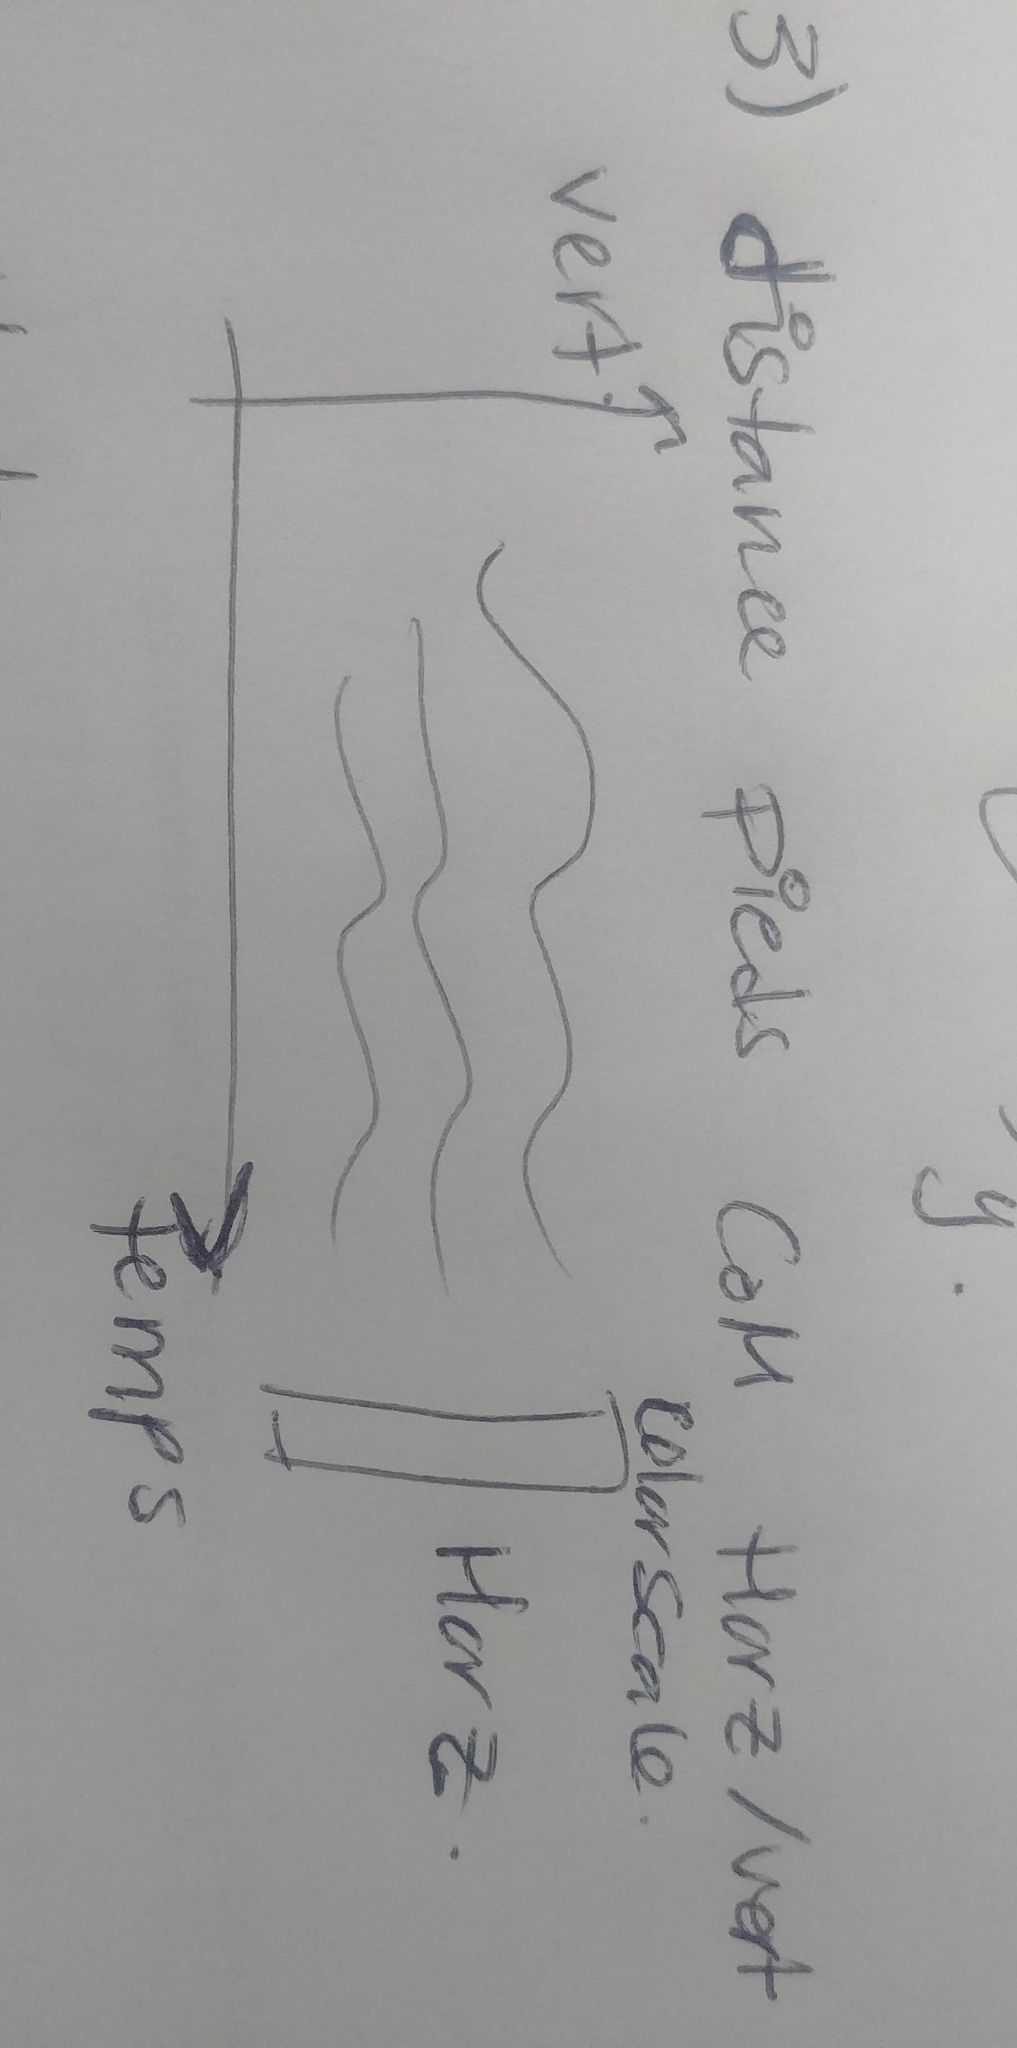
\includegraphics[width=0.5\linewidth, angle =90]{figures/ALaMain_1.jpg}
\label{fig:fig1}
\end{figure}

4) \ref{fig:fig2}
\begin{figure}[h!]
\centering
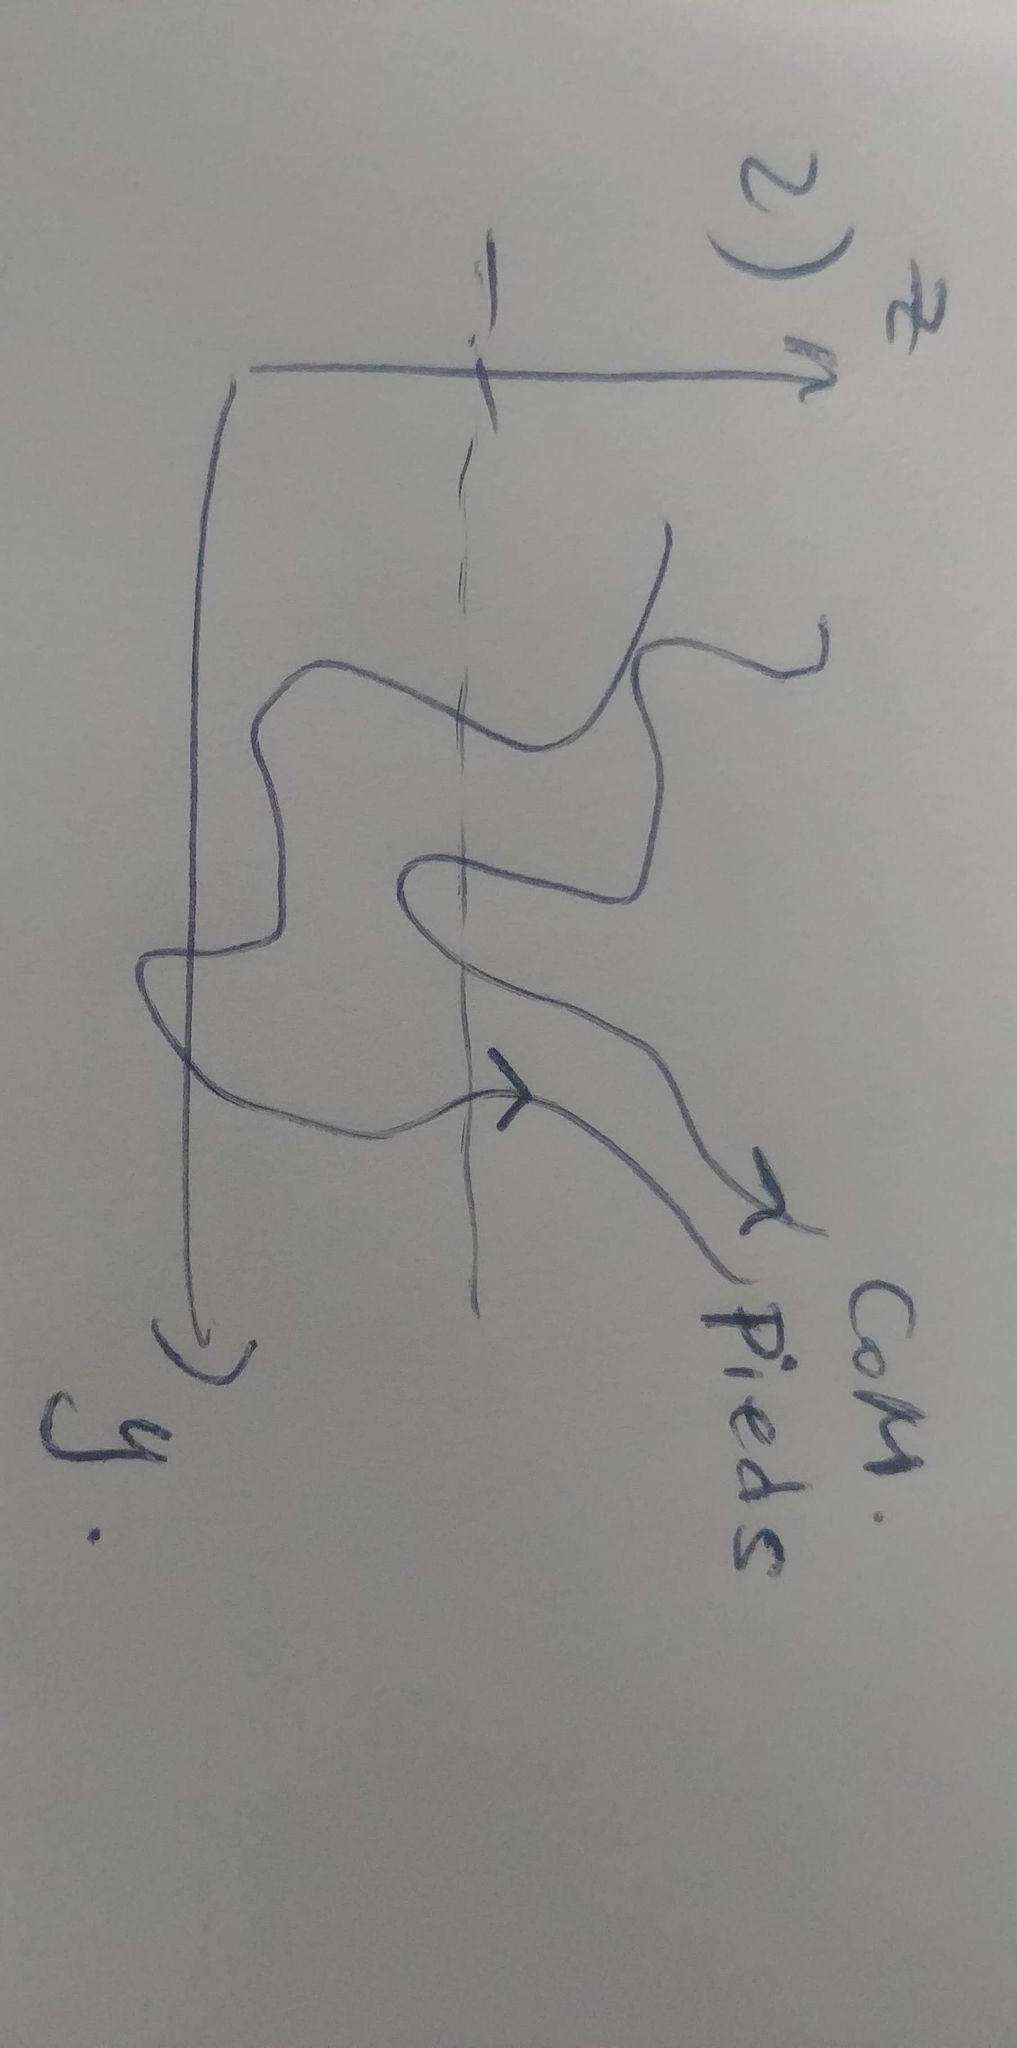
\includegraphics[width=0.5\linewidth, angle =90]{figures/ALaMain_2.jpg}
\label{fig:fig2}
\end{figure}

5) \ref{fig:fig3}
\begin{figure}[h!]
\centering
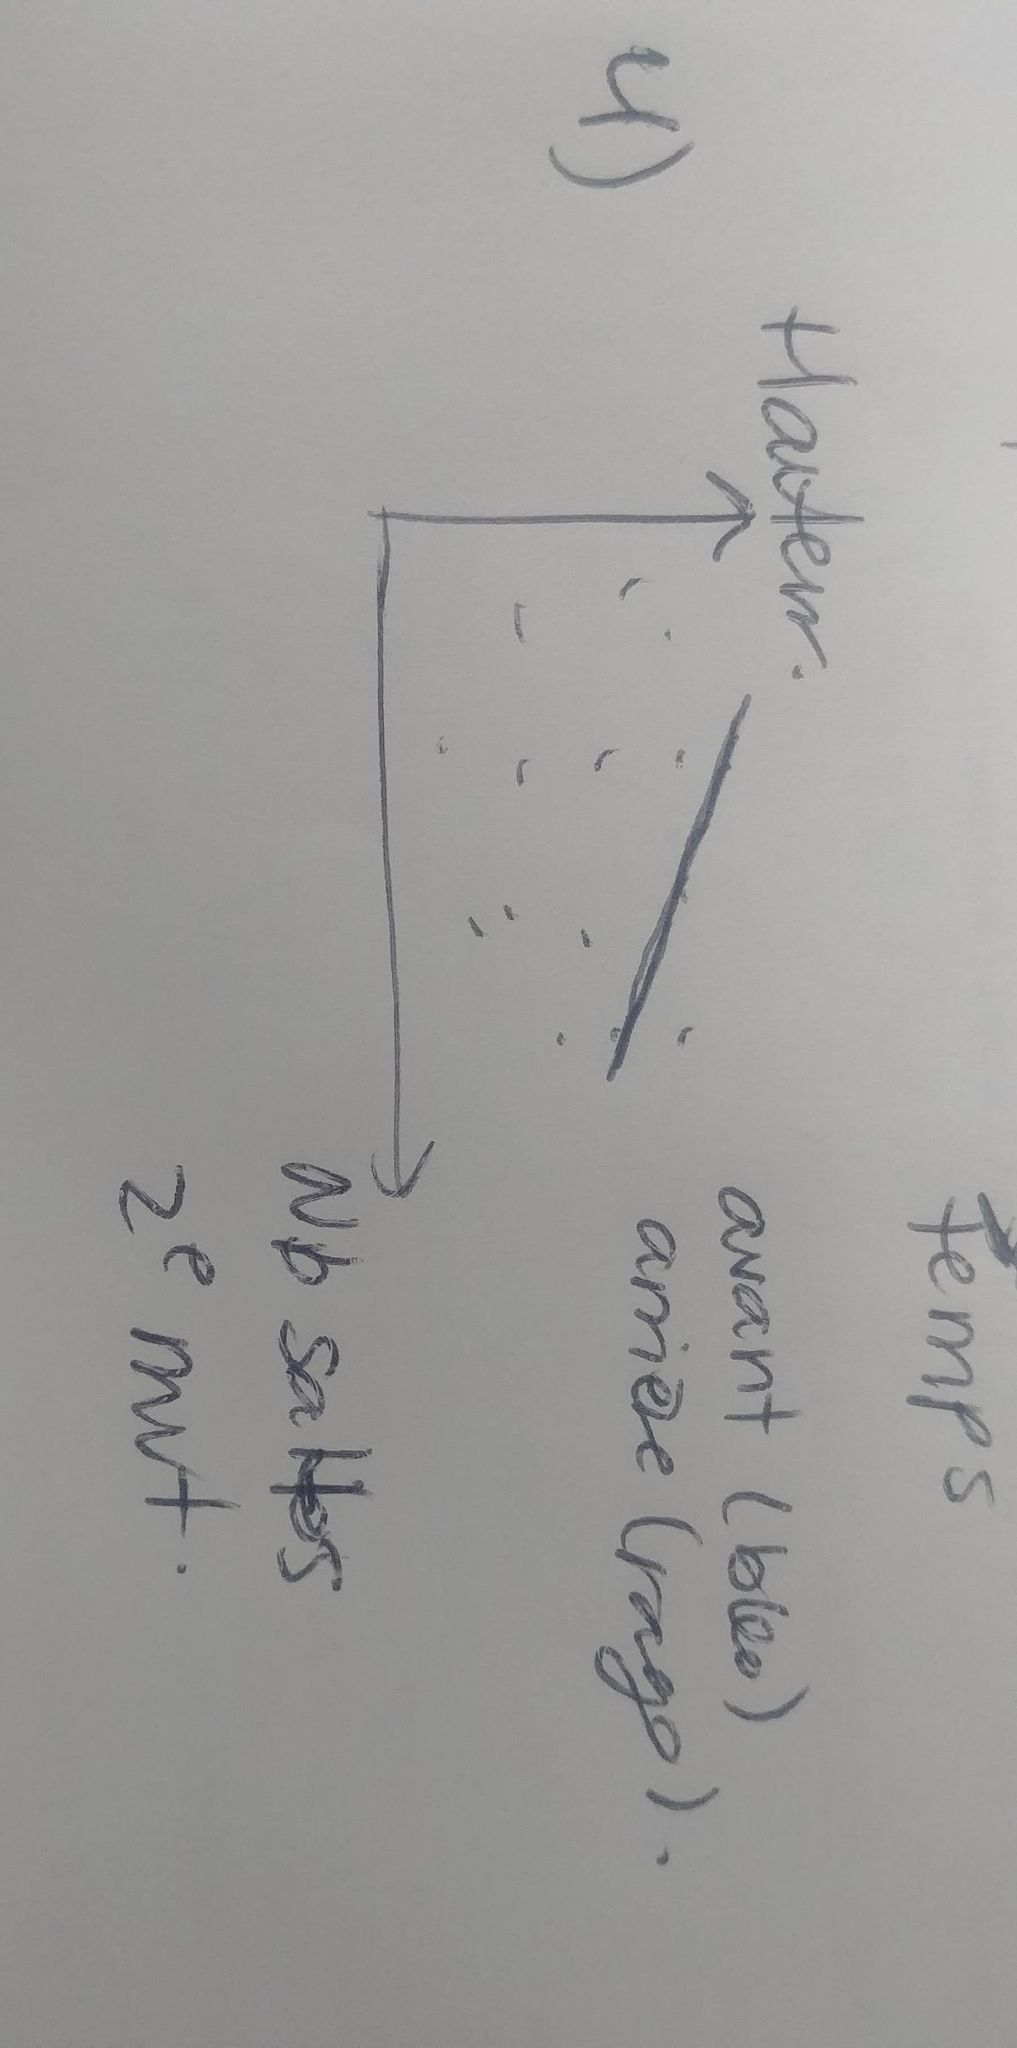
\includegraphics[width=0.5\linewidth, angle =90]{figures/ALaMain_3.jpg}
\label{fig:fig3}
\end{figure}

6) bras de levier au cours du temps (déplacement toile horz 1 grandeur de la force au cours du contact)

7) Travail vertical et horz en fct du nb de saltos

Aussi
convergence rate.
Est-ce que les torques hit les bounds.

